%version 1.00,	date 12/05/2016	auteur(s) Pierre Porche
\speaker{\Julie}

\begin{frame}
\frametitle{Aide à l'attribution des interventions}
	\begin{minipage}[c]{.40\linewidth}
      \begin{figure}[r]
		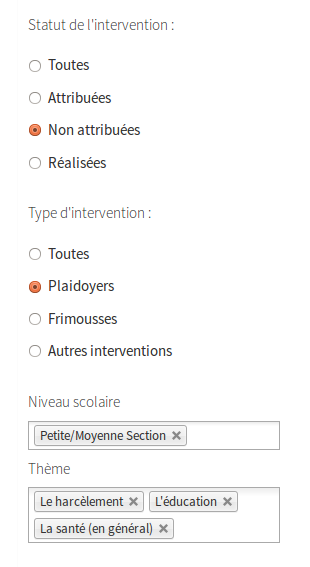
\includegraphics[scale=0.35]{images/filtreListeIntervention.png}
		%\caption{Imprim-écran des possibilités de tris}
	  \end{figure}
   \end{minipage} \hfill
   \begin{minipage}[c]{.52\linewidth}
      \begin{block}{Les filtres}
		\begin{itemize}
			\item requêtes sur la base de données
			\item notion de \texttt{Repository}
		\end{itemize}
	  \end{block}
	  \begin{block}{Rôle des \texttt{Repository}}
		Un repository permet de centraliser tout ce qui touche à la récupération des entités.
		\begin{itemize}
		\item \texttt{class} PHP
		\item \texttt{extends EntityRepository}
		\end{itemize}
	  \end{block}
   \end{minipage} \hfill
\end{frame}

\begin{frame}
	\begin{block}{Les méthodes de récupération des entités}
		\begin{itemize}
			\item méthodes de récupération de base : \\
			 \texttt{find, findAll, findBy, findOneBy, findByX, findOneByX}
			\item méthodes de récupération personnelle : \\
			\texttt{DQL} et \texttt{Query Builder}
		\end{itemize}
	  \end{block}
\end{frame}
